% AL: This is an alternate version of Lecture 02 developed by Andre.
% It would be good to merge this into a single lecture. I prefer the
% example used in the main version since it is close to (hopefully
% identical) to the first example in the FEniCS Tutorial.

\documentclass{fenicscourse}
% General math notation
\newcommand{\N}{\mathbb{N}}
\newcommand{\PP}{\mathbb{P}}
\newcommand{\QQ}{\mathbb{Q}}

% Math operators
\DeclareMathOperator{\ord}{ord}
\DeclareMathOperator{\Kern}{ker}
\DeclareMathOperator{\Image}{im}
\DeclareMathOperator{\spann}{span}
\DeclareMathOperator{\diam}{diam}


% Mesh and FEM notation
%\newcommand{\dx}{\, \mathrm{d} x}
%\newcommand{\ds}{\, \mathrm{d} s}
%\newcommand{\dS}{\, \mathrm{d} S}
\newcommand{\mesh}{\mathcal{T}}
\newcommand{\facets}{\mathcal{F}}
\newcommand{\inmesh}{\partial_i \mathcal{T}}
\newcommand{\exmesh}{\partial_e \mathcal{T}}

\newcommand{\jump}[1]{\llbracket #1 \rrbracket}
\newcommand{\avg}[1]{\langle #1 \rangle}
\newcommand{\meanvalue}[1]{\langle #1 \rangle}
\newcommand{\vect}[1]{\mathbf{#1}}

\newcommand{\gradhterm}[2]{(\nabla_h #1, \nabla_h #2)_{\Omega}}
\newcommand{\consterm}[2]{(\avg{\nabla_h #1} \dotn,\jump{#2})_{\inmesh}}
\newcommand{\penterm}[2]{( h^{-1} \jump{#1}, \jump{#2})_{\inmesh}}

\newcommand{\Ctr}{C_{\text{tr}}}

% Abbreviations for names etc
\newcommand{\apriori}{\emph{a~priori}}
\newcommand{\aposteriori}{\emph{a~posteriori}}

% Dimensions
\newcommand{\codesize}{\footnotesize}

% Environments
\DefineVerbatimEnvironment{code}{Verbatim}{frame=single,rulecolor=\color{blue}}

% Notes
\newcommand{\amnote}[1]{\todo[inline,color=blue!40]{\underline{AM:} #1}}
\newcommand{\mglnote}[1]{\todo[inline,color=red!40]{\underline{MGL:} #1}}
\newcommand{\alnote}[1]{\todo[inline,color=green!40]{\underline{AL:} #1}}
\newcommand{\mernote}[1]{\todo[inline,color=pink!40]{\underline{MER:} #1}}

% Special notation PI
\newcommand{\OmegaD}{\Omega_{0,\mathrm{D}}}
\newcommand{\OmegaN}{\Omega_{0,\mathrm{N}}}
\newcommand{\OmegaO}{\Omega_{_\mathrm{O}}}
\newcommand{\bfsigma}{{\pmb\sigma}}
\newcommand{\bfepsilon}{{\pmb\epsilon}}

% Special notation for PII
\newcommand{\bfu}{\boldsymbol{u}}
\newcommand{\bff}{\boldsymbol{f}}
\newcommand{\bfg}{\boldsymbol{g}}
\newcommand{\bfv}{\boldsymbol{v}}
\newcommand{\bfe}{\boldsymbol{e}}
\newcommand{\bfn}{\boldsymbol{n}}
\newcommand{\bfx}{\boldsymbol{x}}
\newcommand{\Oast}{\Omega^{\ast}}
\newcommand{\Vast}{\mathcal{V}^{\ast}}

%\newcommand{\meshast}{\mathcal{T}_{\ast}}
\newcommand{\pO}{\partial \Omega}
\newcommand{\meshast}{\mathcal{T}^{\ast}}
\newcommand{\Fast}{\mathcal{F}^{\ast}_{\Gamma}}
\newcommand{\piast}{\pi^{\ast}_h}
\newcommand{\tnast}{\tn_{\ast}}
\newcommand{\tnsip}{\tn_{\text{sip}}}
\newcommand{\tnsipast}{\tn_{\text{sip},\ast}}
\newcommand{\asip}{a^{\text{sip}}_h}

\newcommand{\mcF}{\mathcal{F}}
\newcommand{\mcT}{\mathcal{T}}
\newcommand{\mcV}{\mathcal{V}}
\newcommand{\mcE}{\mathcal{E}}
\newcommand{\mcN}{\mathcal{N}}
\newcommand{\mcC}{\mathcal{C}}
\newcommand{\mcA}{\mathcal{A}}
\newcommand{\tn}{|\mspace{-1mu}|\mspace{-1mu}|}
\newcommand{\Pzero}{P_h^{0,\mathrm{dc}}}
\newcommand{\Pone}{P_h^1}
\newcommand{\ndot}{\bfn \cdot}
\newcommand{\dotn}{\cdot \bfn}
\newcommand{\bfw}{\boldsymbol{w}}
\newcommand{\Wspace}{{\mathcal{V}_h}}

% Special notation for PIII
\newcommand{\nablan}{\partial_{\bfn}}
\newcommand{\OmcupOm}{\Omega_1 \cup \Omega_2}
\newcommand{\mcupm}{{\mathcal{T}^{\ast}_1} \cup \mesh_2}
%\newcommand{\mcupm}{{\meshast}_1 \cup \mesh_2}
%\newcommand{\meanvalue}[1]{\langle #1 \rangle_{\alpha}}
\newcommand{\ifnormalpha}[1]{\ifnorm{#1}{\alpha}}
\newcommand{\ifnorm}[2]{\| #1 \|_{#2,h,\Gamma}}
\newcommand{\tildev}{\widetilde{\bfv}}
\newcommand{\bfphi}{\boldsymbol{\phi}}
\newcommand{\picorr}{\pi^c}

% Math macros
\newcommand{\renni}[2]{\langle #2 ,\; #1 \rangle}


\begin{document}

\fenicslecture{Lecture 2: Static linear PDEs}
              {Hans Petter Langtangen \\
               Anders Logg\\
               Andr\'e Massing}


\begin{frame}
  \frametitle{Hello World!}

  We will solve Poisson's equation, the Hello World of scientific
  computing:
  \begin{equation*}
    \begin{split}
      - \Delta u &= f \,\,\, \quad \mbox{in } \Omega
      \\
    u &= u_0 \quad \mbox{on } \partial \Omega
    \end{split}
  \end{equation*}

  Poisson's equation arises in numerous contexts:
  \begin{itemize}
  \item
    heat conduction, electrostatics, diffusion
    of substances, twisting of elastic rods, inviscid fluid flow, water
    waves, magnetostatics
  \item
    as part of numerical splitting strategies of more complicated
    systems of PDEs, in particular the Navier--Stokes equations
  \end{itemize}

\end{frame}

\begin{frame}
  \frametitle{The FEM cookbook}

  \def\svgwidth{1.05\textwidth}
  \import{pdf/}{pdf/fem_steps.pdf_tex}

\end{frame}

\begin{frame}
  \frametitle{Solving PDEs in FEniCS}

  Solving a physical problem with FEniCS consists of the following steps:
  \begin{enumerate}
  \item
    Identify the PDE and its boundary conditions
  \item
    Reformulate the PDE problem as a variational problem
  \item
    Make a Python program where the formulas in the variational
    problem are coded, along with definitions of input data such as $f$,
    $u_0$, and a mesh for $\Omega$
  \item
    Add statements in the program for solving the variational problem,
    computing derived quantities such as $\nabla u$, and visualizing
    the results
  \end{enumerate}

\end{frame}

\begin{frame}
  \frametitle{Deriving a variational problem for Poisson's equation}

  The simple recipe is: multiply the PDE by a test function $v$ and
  integrate over $\Omega$:
  \begin{equation*}
    -\int_\Omega (\Delta u)v \dx = \int_\Omega fv\dx
  \end{equation*}

  Then integrate by parts and set $v = 0$ on the Dirichlet boundary:

  \begin{equation*}
    -\int_\Omega (\Delta u) v \dx
    = \int_\Omega \nabla u\cdot\nabla v\dx -
   \underbrace{\int_{\partial\Omega} \frac{\partial u}{\partial n} v\ds}_{\textcolor{fenicsred}{=0}}
  \end{equation*}

  We find that:
  \begin{equation*}
    \int_\Omega\nabla u\cdot\nabla v\dx = \int_\Omega fv\dx
  \end{equation*}

\end{frame}

\begin{frame}
  \frametitle{Variational problem for Poisson's equation}

  Find $u \in V$ such that
  \begin{equation*}
    \int_{\Omega} \nabla u \cdot \nabla v \dx =
    \int_{\Omega} fv \dx
  \end{equation*}
  for all $v \in \hat{V}$

  \bigskip

  The trial space $V$ and the test space $\hat{V}$ are (here)
  given by
  \begin{equation*}
    \begin{split}
      V       &= \{v \in H^1(\Omega) : v = u_0 \mbox{ on } \partial\Omega\} \\
      \hat{V} &= \{v \in H^1(\Omega) : v = 0 \mbox{ on } \partial\Omega\}
    \end{split}
  \end{equation*}

\end{frame}

\begin{frame}
  \frametitle{Discrete variational problem for Poisson's equation}

  We approximate the continuous variational problem with a discrete
  variational problem posed on finite dimensional subspaces of $V$ and $\hat{V}$:

  \begin{align*}
    V_h &\subset V \\
    \hat{V}_h &\subset \hat{V}
  \end{align*}

  \bigskip

  Find $u_h \in V_h \subset V$ such that
  \begin{equation*}
    \int_{\Omega} \nabla u_h \cdot \nabla v \dx =
    \int_{\Omega} fv \dx
  \end{equation*}
  for all $v \in \hat{V}_h \subset \hat{V}$

\end{frame}

\begin{frame}
  \frametitle{Canonical variational problem}

  The following canonical notation is used in FEniCS: find
  $u \in V$ such that
  \begin{equation*}
    a(u, v) = L(v)
  \end{equation*}
  for all $v \in \hat{V}$

  \bigskip

  For Poisson's equation, we have
  \begin{align*}
    a(u, v) &= \int_{\Omega} \nabla u \cdot \nabla v \dx
    \\
    L(v) &= \int_{\Omega} fv \dx
  \end{align*}

  \bigskip
  $a(u, v)$ is a \emph{bilinear form} and $L(v)$ is a \emph{linear form}

\end{frame}


\begin{frame}
  \frametitle{Poisson example 1}
  \begin{block}{Strong form}
    Let $\Omega = [0,1]\times[0,1]$. Solve
    \begin{align*}
      -\Delta u &= 1 \quad \text{in } \Omega \\
              u &= 0 \quad \text{on } \partial \Omega
    \end{align*}
  \end{block}
  \vspace{-1em}
  \begin{block}{Weak form}   
    Find $u \in H^1_0(\Omega)$ such that for all $v \in H^1_0(\Omega)$
    \begin{equation*}
      \underbrace{
      \int_{\Omega} \nabla u \cdot \nabla v \dx
    }_{a(u,v)}
        = \underbrace{
          \int_{\Omega} 1 v \dx
        }_{L(v)}
    \end{equation*}
  \end{block}
\end{frame}

\begin{frame}[shrink=20]
%\begin{frame}
  \frametitle{Poisson example 2}
    \begin{itemize}
      \item Domain: \vspace{-1em}
        \begin{align*}
          \Omega &= [0,1]\times[0,1] \\
        \partial \Omega_D &= \{0\} \times [0,1] \cup \{1\} \times
        [0,1]
        \\
        \partial \Omega_N &= [0,1] \times \{0\}  \cup [0,1] \times 
        \{1\}  
        \end{align*}
      \item  Source and boundary values: 
        \vspace{-0.5em}
        \begin{align*}
          f(x,y) &= 2\cos(2\pi x)\cos(2\pi y) 
          \\
          g_D(x,y) &= 0.1 \cos(2\pi y)
        \end{align*}
    \end{itemize}
    \vspace{-1em}
    \begin{columns}[t]
      \begin{column}{0.4\textwidth}
        \begin{block}{Strong form}
          \vspace{-2em}
          \begin{align*}
            -\Delta u &= f \quad \text{in } \Omega \\
                    u &= g_D \quad \text{on } \partial \Omega_D \\
              \dfrac{\partial u}{\partial \bfn} &= 0 \quad \text{on }
            \partial \Omega_N
          \end{align*}
        \end{block}
      \end{column}
      \begin{column}{0.6\textwidth}
        \uncover<2->{
        \begin{block}{Weak form}   
          Find $u \in V$ such that for all $v \in \widehat{V}$
          \begin{equation*}
            \underbrace{
              \int_{\Omega} \nabla u \cdot \nabla v \dx
            }_{a(u,v)}
            = \underbrace{
              \int_{\Omega} f v \dx
            }_{L(v)}
          \end{equation*}
        \end{block}
      }
      \end{column}
    \end{columns}
    \uncover<2->{
    \begin{itemize}
      \item Function spaces: \vspace{-1em}
        \begin{equation*}
          \begin{split}
            V       &= \{v \in H^1(\Omega) : v = g_D \mbox{ on }
          \partial\Omega_D\} \\
            \hat{V} &= \{v \in H^1(\Omega) : v = 0 \mbox{ on }
        \partial\Omega_D\}
          \end{split}
        \end{equation*}
    \end{itemize}
  }
  \end{frame}

\begin{frame}[shrink=20]
  \frametitle{Poisson example 3}
    \begin{itemize}
      \item Domain: \vspace{-1em}
        \begin{align*}
            \Omega &= [0,1]\times[0,1] \setminus \text{dolphin domain} \\
        \partial \Omega_D &= \{0\} \times [0,1] \cup \{1\} \times
        [0,1]
        \\
        \partial \Omega_N &= \partial \Omega \setminus \partial
        \Omega_D
        \end{align*}
      \item  Source and boundary values: 
        \vspace{-0.5em}
        \begin{align*}
          f(x,y) &= 2\cos(2\pi x)\cos(2\pi y) 
          \\
          g_D(x,y) &= 0.5 \cos(2\pi y) \quad \text{on } x = 0 \\
          g_D(x,y) &= 1 \quad \text{on } x = 1 \\
          g_N(x,y) &= \sin(\pi x)\sin(\pi y)
        \end{align*}
    \end{itemize}
    \vspace{-1em}
    \begin{columns}[t]
      \begin{column}{0.4\textwidth}
        \begin{block}{Strong form}
          \vspace{-2em}
          \begin{align*}
            -\Delta u &= f \quad \text{in } \Omega \\
                    u &= g_D \quad \text{on } \partial \Omega_D \\
              -\dfrac{\partial u}{\partial \bfn} &= g_N \quad \text{on }
            \partial \Omega_N
          \end{align*}
        \end{block}
      \end{column}
      \begin{column}{0.6\textwidth}
        \uncover<2->{
        \begin{block}{Weak form}   
          Find $u \in V$ such that for all $v \in \widehat{V}$
          \begin{equation*}
            \underbrace{
              \int_{\Omega} \nabla u \cdot \nabla v \dx
            }_{a(u,v)}
            = \underbrace{
                \int_{\Omega} f v \dx + \int_{\partial \Omega_N} g v
                \ds
            }_{L(v)}
          \end{equation*}
        \end{block}
      }
      \end{column}
    \end{columns}
    \uncover<2->{
    \begin{itemize}
      \item Function spaces: \vspace{-1em}
        \begin{equation*}
          \begin{split}
            V       &= \{v \in H^1(\Omega) : v = g_D \mbox{ on }
          \partial\Omega_D\} \\
            \hat{V} &= \{v \in H^1(\Omega) : v = 0 \mbox{ on }
        \partial\Omega_D\}
          \end{split}
        \end{equation*}
    \end{itemize}
  }
  \end{frame}

\begin{frame}[fragile,shrink=10]
    \frametitle{Poisson example 3: Mission possible}
    \begin{block}{Your mission}
        \begin{itemize}
            \item open and plot the dolfin mesh saved in
                dolfin-channel.xml
            \item solve the discrete variational problem
            \item export the solution to a pvd file and visualize
                it in Paraview
        \end{itemize}
    \end{block}
    \begin{block}{Your tools}
            Read in a mesh
            \vspace{-1em}
        \begin{python}
mesh = Mesh("dolfin-channel.xml")
        \end{python}
        Inhomogeneus Neuman boundary condition
        \vspace{-1em}
        \begin{python}
L = ... + g_N*v*ds
        \end{python}
        List of Dirchlet boundary conditions
        \vspace{-1em}
        \begin{python}
            bc0 = DirichletBC(...)
            bc1 = DirichletBC(...)
            bcs = [bc0, bc1]
        \end{python}
        Save solution in VTK format
        \vspace{-1em}
        \begin{python}
u_file = File("poisson_3.pvd")
u_file << u
        \end{python}
    \end{block}
\end{frame}

\begin{frame}
    \frametitle{Poisson example 3: Extra mission}
    \begin{itemize}
        \item Choose a variable \colemph{conductivity} of the form
            \begin{equation*}
                k(x,y) = 1 + e^{(x^2 + y^2)}
            \end{equation*}
        \item What is the expression of the heat flux $\sigma$ across the
            boundary now (opposed to 
            $\sigma  \cdot \bfn = \tfrac{\partial u}{\partial \bfn}$ in the
            original problem)? 
        \item Replace the inhomogeneus Neumann boundary condition by a
            Robin boundary condition
            \begin{equation*}
                -\sigma \cdot \bfn = u - g_N \quad \text{on } \partial
                \Omega_N
            \end{equation*}
        \item
            Solve
            \vspace{-2em}
            \begin{align*}
                -\nabla \cdot (k(x,y) \nabla u ) &= f \quad \text{in } \Omega \\
                                               u &= g_D \quad \text{on } \partial \Omega_D \\
                               -\sigma \cdot \bfn &= u - g_N \quad \text{on }
                \partial \Omega_N
            \end{align*}
            by finding the weak formulation of the problem and solving it
            using \texttt{FEniCS}
    \end{itemize}
\end{frame}

%\input{slides/compute_gradient_1.tex}
\begin{frame}[shrink=20]
  \frametitle{Poisson example 4}
    \begin{itemize}
      \item Domain: \vspace{-1em}
        \begin{align*}
            \Omega_1 &= [0,1]\times[0,0.5] 
            \\
            \Omega_2 &= [0,1]\times[0.5,1] 
            \\
            \Omega &= \Omega_1 \cup \Omega_2 \\
        \partial \Omega_D &= \partial \Omega
        \end{align*}
      \item  Conductivity, source and boundary values: 
        \vspace{-0.5em}
        \begin{align*}
            k(x,y) &= 
            \begin{cases}
                10 &\quad \text{in } \Omega_1  \\ 
                50 + e^{50(0.5 - y )^2} &\quad \text{in } \Omega_2
            \end{cases}
            \\
          f(x,y) &= 1
          \\
          g_D(x,y) &= 0 
        \end{align*}
    \end{itemize}
    \vspace{-1em}
    \begin{columns}[t]
      \begin{column}{0.5\textwidth}
        \begin{block}{Strong form}
          \vspace{-2em}
          \begin{align*}
            -\nabla \cdot (k_1(x,y) \nabla u) &= f \quad \text{in } \Omega_1 \\
            -\nabla \cdot (k_2(x,y) \nabla u) + u  &= f \quad \text{in } \Omega_2 \\
                    u &= g_D \quad \text{on } \partial \Omega_D \\
          \end{align*}
        \end{block}
      \end{column}
      \begin{column}{0.5\textwidth}
        \uncover<2->{
        \begin{block}{Weak form}   
          Find $u \in V$ such that for all $v \in \widehat{V}$
          \begin{equation*}
            \underbrace{
              \int_{\Omega_1} k_1 \nabla u \cdot \nabla v \dx
             +\int_{\Omega_2} k_2 \nabla u \cdot \nabla v  + uv \dx
            }_{a(u,v)}
            = \underbrace{
                \int_{\Omega} f v \dx
            }_{L(v)}
          \end{equation*}
        \end{block}
      }
      \end{column}
    \end{columns}
    \uncover<2->{
    \begin{itemize}
      \item Function spaces: \vspace{-1em}
        \begin{equation*}
          \begin{split}
            V       &= \{v \in H^1(\Omega) : v = g_D \mbox{ on }
          \partial\Omega_D\} \\
            \hat{V} &= \{v \in H^1(\Omega) : v = 0 \mbox{ on }
        \partial\Omega_D\}
          \end{split}
        \end{equation*}
    \end{itemize}
  }
  \end{frame}

%\input{slides/poisson_4_exercise.tex}
\begin{frame}[shrink=35]
%\begin{frame}
  \frametitle{The FEniCS challenge!}
  \begin{columns}[c]
    \begin{column}{0.5\textwidth}
      \begin{itemize}
        \item Domain: \vspace{-1em}
          \begin{align*}
            \Omega_{_{DO}} &= \text{dolphin domain} \\
                    \Omega &= [0,1]\times[0,1] \setminus \Omega_{_{DO}} \\
                    \Omega_1 &= \{ T \in \mesh : T \subset
          B_{0.35}(0.5,0.5) \} \\
            \Omega_2 &= \Omega \setminus \Omega_1 \\
            \partial \Omega_D &= \{0\} \times [0,1] \cup \{1\} \times
            [0,1]
            \\
            \partial \Omega_{N,1} &= \partial \Omega_{_{DO}} \\
            \partial \Omega_{N,2} &= [0,1] \times \{0\} \cup
            [0,1] \times \{1\}               
          \end{align*}
        \item  Conductivity, source and boundary values: 
          \vspace{-0.5em}
          \begin{align*}
            k(x,y) &= 
            \begin{cases}
              10 &\quad \text{in } \Omega_1  \\ 
      50 + e^{50(0.5 - y )^2} &\quad \text{in } \Omega_2
            \end{cases}
            \\
            f(x,y) &= 1
            \\
            g_D(x,y) &= 0 \\
        g_{N,1}(x,y) &= 0 \\
        g_{N,2}(x,y) &= \sin(\pi x)\sin(\pi y)
          \end{align*}
        \item As an alternative, reuse the source function and the
          Dirichlet boundary values from exercise 3:
          \begin{align*}
            f(x,y) &= 2\cos(2\pi x)\cos(2\pi y) 
            \\
            g_D(x,y) &= 0.5 \cos(2\pi y) \quad \text{on } x = 0 \\
            g_D(x,y) &= 1 \quad \text{on } x = 1 \\
          \end{align*}
      \end{itemize}
    \end{column}
    \begin{column}{0.5\textwidth}
      \begin{center}
        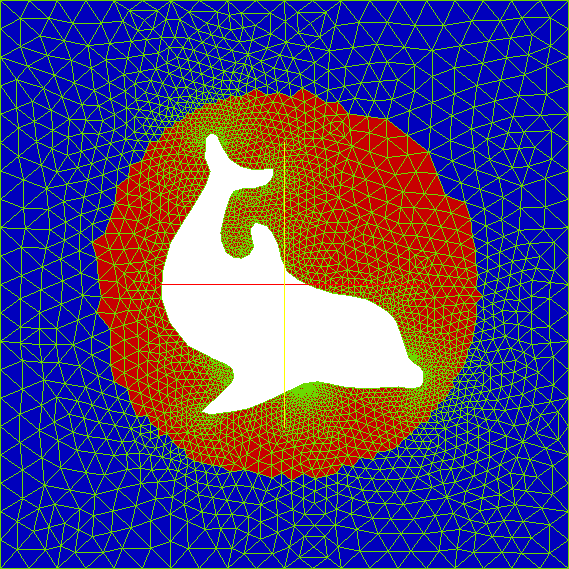
\includegraphics[width=1.0\textwidth]{png/poisson_5_subdomains.png}
      \end{center}
    \end{column}
  \end{columns}
\end{frame}


\begin{frame}[shrink=20,fragile]
  \frametitle{The FEniCS challenge!}
  \begin{columns}[c]
    \begin{column}{0.5\textwidth}
    Solve
          \vspace{-1em}
          \begin{align*}
            -\nabla \cdot (k_1(x,y) \nabla u) + u  &= f \quad \text{in
          } \Omega_1 \\
            -\nabla \cdot (k_2(x,y) \nabla u) &= f \quad \text{in }
              \Omega_2 
          \end{align*}
          \vspace{-2.0em}
          \begin{align*}
                    u &= g_D \quad \text{on } \partial \Omega_D \\
            -\dfrac{\partial u}{\partial \bfn} &= g_{N,1} \quad \text{on }
            \partial \Omega_{N,1} \\
            -\dfrac{\partial u}{\partial \bfn} &= u - g_{N,2} \quad \text{on }
            \partial \Omega_{N,2}
          \end{align*}
    by first finding the weak formulation and then solving the system
    numerically using \text{FEniCS}
    \end{column}
    \begin{column}{0.5\textwidth}
      \begin{center}
        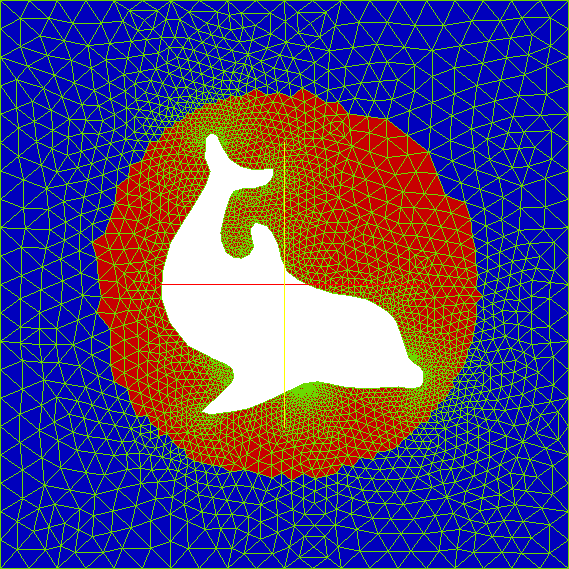
\includegraphics[width=1.0\textwidth]{png/poisson_5_subdomains.png}
      \end{center}
    \end{column}
  \end{columns}
  \begin{block}{Tools}
    Define facet markers
    \vspace{-1em}
    \begin{python}
boundary_markers = FacetFunction("size_t",mesh)
...
    \end{python}
    A redefinition of ``ds'' is necessary as well (why?). How will that probably look
    like? 
\end{block}
\end{frame}


%Code verification
%interpolate


%\begin{frame}
  \frametitle{A test problem}

  We construct a test problem for which we can easily check the
  answer. We first define the exact solution by
  \begin{equation*}
    u(x, y) = 1 + x^2 + 2y^2
  \end{equation*}

  \bigskip

  We insert this into Poisson's equation:

  \begin{equation*}
     f = -\Delta u = -\Delta (1 + x^2 + 2y^2) = -(2 + 4) = -6
  \end{equation*}

  \bigskip

  This technique is called the \emph{method of manufactured solutions}

\end{frame}

%\begin{frame}[fragile]
  \frametitle{Implementation in FEniCS}

  % This is d1_p2D.py from the FEniCS Tutorial with some minor changes:
  % - comments removed
  % - moved definition of f before u and v
  % - last lines removed

  \begin{python}
from fenics import *

mesh = UnitSquareMesh(6, 4)
V = FunctionSpace(mesh, "Lagrange", 1)
u0 = Expression("1 + x[0]*x[0] + 2*x[1]*x[1]", degree=2)

def u0_boundary(x, on_boundary):
    return on_boundary

bc = DirichletBC(V, u0, u0_boundary)

f = Constant(-6.0)
u = TrialFunction(V)
v = TestFunction(V)
a = inner(grad(u), grad(v))*dx
L = f*v*dx

u = Function(V)
solve(a == L, u, bc)
  \end{python}

% Last part of the program does not fit on page
%plot(u)
%plot(mesh)
%
%file = File("poisson.pvd")
%file << u
%
%interactive()

\end{frame}

%\begin{frame}[fragile]
  \frametitle{Step by step: the first line}

  The first line of a FEniCS program usually begins with

  \begin{python}
from fenics import *
  \end{python}

  \bigskip

  This imports key classes like \emp{UnitSquareMesh}, \emp{FunctionSpace},
  \emp{Function} and so forth, from the FEniCS user interface
  (DOLFIN)

\end{frame}

%\begin{frame}[fragile]
  \frametitle{Step by step: creating a mesh}

  Next, we create a mesh of our domain $\Omega$:
  \vspace{-1em}
  \begin{python}
mesh = UnitSquareMesh(8, 8)
  \end{python}
  This defines a mesh of $8 \times 8 \times 2 = 128$ triangles of the
  unit square.

  \bigskip

  Other useful classes for creating built-in meshes include
  \emp{UnitIntervalMesh},
  \emp{UnitCubeMesh},
  \emp{UnitCircleMesh},
  \emp{UnitSphereMesh},
  \emp{RectangleMesh} and
  \emp{BoxMesh}

  \bigskip

  More complex geometries can be built using Constructive Solid
  Geometry (CSG) through the FEniCS component \emp{mshr}:
  \vspace{-1em}
  \begin{python}
from mshr import *
r = Rectangle(Point(0.5, 0.5), Point(1.5, 1.5))
c = Circle(Point(1.0, 1.0), 0.2)
g = r - c
mesh = generate_mesh(g, 10)
  \end{python}

  \normalsize

\end{frame}

%\begin{frame}[fragile]
  \frametitle{Step by step: creating a function space}

  The following line creates a finite element function space relative to this mesh:
\vspace{-1em}
\begin{python}
V = FunctionSpace(mesh, "Lagrange", 1)
\end{python}

  \bigskip

  The second argument specifies the type of element, while the third
  argument is the degree of the basis functions on the element

  \bigskip

  Other types of elements include
  \emp{"Discontinuous Lagrange"},
  \emp{"Brezzi-Douglas-Marini"},
  \emp{"Raviart-Thomas"},
  \emp{"Crouzeix-Raviart"},
  \emp{"Nedelec 1st kind H(curl)"} and
  \emp{"Nedelec 2nd kind H(curl)"}

\end{frame}

%\begin{frame}[fragile]
  \frametitle{Step by step: defining expressions}

  Next, we define an expression for the boundary value:
  \vspace{-1em}
  \begin{python}
u0 = Expression("1 + x[0]*x[0] + 2*x[1]*x[1]", degree=2)
  \end{python}
  The formula must be written in C++ syntax, and
  the polynomial degree must be specified.

  \bigskip

  The \emp{Expression} class is very flexible and can be used to
  create complex user-defined expressions. For more information, try
\vspace{-1em}
  \begin{python}
from fenics import *
help(Expression)
  \end{python}
  in Python or, in the shell:
  \vspace{-1em}
  \begin{python}
$ pydoc fenics.Expression
  \end{python}

\end{frame}

%\begin{frame}[fragile]
  \frametitle{Step by step: defining boundaries}

  We next define the Dirichlet boundary:
  \vspace{-0.25cm}
\begin{python}
def u0_boundary(x, on_boundary):
    return on_boundary
\end{python}

  \bigskip

  You may want to experiment with the definition of the boundary:

\begin{python}
def u0_boundary(x):
    return x[0] < DOLFIN_EPS or \
           x[1] > 1.0 - DOLFIN_EPS
\end{python}
\vspace{-0.5cm}
\begin{python}
def u0_boundary(x):
    return near(x[0], 0.0) or near(x[1], 1.0)
\end{python}
\vspace{-0.5cm}
\begin{python}
def u0_boundary(x, on_boundary):
    return on_boundary and x[0] > DOLFIN_EPS
\end{python}

\end{frame}

%\begin{frame}[fragile]
  \frametitle{Step by step: defining a boundary condition}

  The following code defines a Dirichlet boundary condition:

\begin{python}
bc = DirichletBC(V, u0, u0_boundary)
\end{python}

  \bigskip

  This boundary condition states that a function in the function space
  defined by \emp{V} should be equal to \emp{u0} on the boundary
  defined by \emp{u0\_boundary}

  \bigskip

  Note that the above line does not yet apply the boundary condition
  to all functions in the function space

\end{frame}

%\begin{frame}[fragile]
  \frametitle{Step by step: defining the right-hand side}

  The right-hand side $f = - 6$ may be defined as follows:
  \begin{python}
f = Expression("-6.0", degree=0)
  \end{python}

  \bigskip

  or (more efficiently) as
  \begin{python}
f = Constant(-6.0)
  \end{python}

\end{frame}

%\begin{frame}[fragile]
  \frametitle{Step by step: defining variational problems}

  Variational problems are defined in terms of \emph{trial} and
  \emph{test} functions:
  \begin{python}
u = TrialFunction(V)
v = TestFunction(V)
  \end{python}

  \bigskip

  We now have all the objects we need in order to specify the bilinear
  form $a(u,v)$ and the linear form $L(v)$:
  \begin{python}
a = inner(grad(u), grad(v))*dx
L = f*v*dx
  \end{python}

\end{frame}

%\begin{frame}[fragile]
  \frametitle{Step by step: solving variational problems}

  Once a variational problem has been defined, it may be solved
  by calling the \emp{solve} function:

  \begin{python}
u = Function(V)
solve(a == L, u, bc)
  \end{python}

  \bigskip

  Note the reuse of the variable name \emp{u} as both a \emp{TrialFunction}
  in the variational problem and a \emp{Function} to store the solution.

\end{frame}

%\begin{frame}[fragile]
  \frametitle{Step by step: post-processing}

  The solution and the mesh may be plotted by simply calling:
  \vspace{-0.25cm}
  \begin{python}
plot(u)
plot(mesh)
interactive()
  \end{python}

  \bigskip

  The \emp{interactive()} call is necessary for the plot to remain on the
  screen and allows the plots to be rotated, translated and zoomed

  \bigskip

  For postprocessing in ParaView or MayaVi, store the solution in VTK
  format:
  \begin{python}
file = File("poisson.pvd")
file << u
  \end{python}

\end{frame}


%\begin{frame}
  \frametitle{\emph{The FEniCS challenge!}}

  Solve the partial differential equation
  \begin{equation*}
    -\Delta u = f
  \end{equation*}
  with homogeneous Dirichlet boundary conditions on the unit square
  for $f(x, y) = 2\pi^2\sin(\pi x)\sin(\pi y)$. Plot the error in the
  $L^2$ norm as function of the mesh size $h$ for a sequence of
  refined meshes. Try to determine the convergence rate.

  \begin{itemize}
  \item
    \emph{Who can obtain the smallest error?}
  \item
    \emph{Who can compute a solution with an error smaller than
    $\epsilon = 10^{-6}$ in the fastest time?}
  \end{itemize}

  \emph{The best students(s) will be rewarded with a FEniCS surprise!}

  \bigskip
  Hints: \emp{help(errornorm)}, \emp{help(assemble)}

\end{frame}


\end{document}
